% vim: set foldmethod=marker foldlevel=0:

\documentclass[a4paper]{article}
\usepackage[UKenglish]{babel}

% NOTE: hyperref has to come before preamble
% \usepackage[hidelinks]{hyperref}

\usepackage{preamble}

\usepackage{tikz}

\fancyhead[L]{MA243 Assignment 2}
\title{MA243 Geometry, Assignment 2}
\colorlet{questionbodycolor}{orange!50}

\begin{document}

\maketitle

\setlength{\parindent}{0em}
\setlength{\parskip}{1em}

% {{{ Q1
\question{1}

\begin{questionbody}
% This question is about geometry in the Euclidean plane, $\R^2$.
%
Let $R_L$ denote the reflection in the line $L$. Let $H_P$ be the rotation through $P$ by $180\degree$. Prove that \[
R_L \circ H_P = H_P \circ R_L \iff P \in L
\]
\end{questionbody}

For the $\Rightarrow$ direction, assume $R_L \circ H_P = H_P \circ R_L$ but suppose $P \notin L$. We can define $P'$ as the point in $L$ which minimises $d(P, P')$, so $P'$ is the perpendicular projection of $P$ onto $L$. Then consider a point $Q$ where $Q$ is closer to $L$ than $P$ is, but on the same side as $P$.

Then $Q_{HR} := (H_P \circ R_L)(Q)$ will be on the same side of $L$ as $P$, but $Q_{RH} := (R_L \circ H_P)(Q)$ will be on the opposite side from $P$.

\begin{figure}[tbph]
\centering
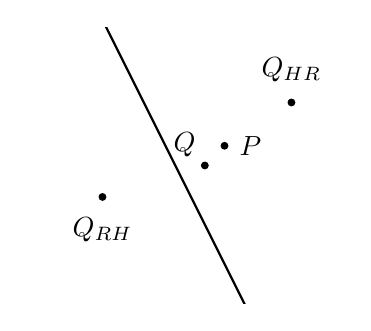
\begin{tikzpicture}[
    scale=5,
]
    \clip (1.6, 0.7) rectangle (2.4, 1.4);
    \begin{scope}[
        every path/.style={thick},
    ]
        \draw (0, 5) -- (3, -1);

        \node[label={[label distance=-2]0:$P$}] (P) at (2.1, 1.1) {};
        \fill (P) circle[radius=0.01];

        \node[label={[label distance=-5]120:$Q$}] (Q) at (2.05, 1.05) {};
        \fill (Q) circle[radius=0.01];

        \node[label=270:$Q_{RH}$] (QRH) at (1.79, 0.97) {};
        \fill (QRH) circle[radius=0.01];

        \node[label=90:$Q_{HR}$] (QHR) at (2.27, 1.21) {};
        \fill (QHR) circle[radius=0.01];
    \end{scope}
\end{tikzpicture}
\caption{A sketch of the situtation}
\end{figure}

Conversely, for the $\Leftarrow$ direction, assume $P \in L$. Without loss of generality, we can work in $\R^2$ and assume $P = (0, 0)$, using an isometry to get to and from any Euclidean space. Since we're in $\R^2$, we can choose a unit vector $\ul v$ in the direction of $L$ and an orthogonal unit vector $\ul u$ with $\ul v \cdot \ul u = 0$. Then $\ul v, \ul u$ is an orthonormal basis, and \[
R_L = \begin{pmatrix} 1 & 0 \\ 0 & -1 \end{pmatrix},
\qquad H_P = \begin{pmatrix} -1 & 0 \\ 0 & -1 \end{pmatrix}
\]

An arbitrary point $Q$ can be written as $\lambda \ul v + \mu \ul u$. Then we can just compute
\begin{align*}
R_L \circ H_P &= R_L(H_P(Q)) \\
&= R_L(H_P(\lambda \ul v + \mu \ul u)) \\
&= R_L(- \lambda \ul v - \mu \ul u) \\
&= - \lambda \ul v + \mu \ul u \\
%
H_P \circ R_L &= H_P(R_L(Q)) \\
&= H_P(R_L(\lambda \ul v + \mu \ul u)) \\
&= H_P(\lambda \ul v - \mu \ul u) \\
&= - \lambda \ul v + \mu \ul u
\end{align*}
These are the same, so $R_L \circ H_P = H_P \circ R_L$.

\hfill $\square$

% }}}

% {{{ Q2
\newquestion{2}

\begin{questionbody}
Define the flat torus to be the metric space given by the set $T := [0, 1) \times [0, 1)$ together with the distance \[ % chktex 9
d((x_1, y_1), (x_2, y_2)) = \min\l\{ d_{\R^2}((x_1, y_1), (x_2 + i, y_2 + j)) : i, j \in \Z \r\}.
\] You can think of this as a square with the top and bottom edges identified, and the left and right sides identified. Here $d_{\R^2}$ is the usual Euclidean metric on $\R^2$. For example, on the flat torus, $(0.9, 0)$ is distance $0.2$ from the point $(0.1, 0)$.

For $z = (x, y) \in \R^2$, define \[ \{z\} = (\{x\}, \{y\}) \] where $\{a\} \in [0, 1)$ is the fractional part of the real number $a$. This is the unique value in $[0, 1)$ such that $a - \{a\}$ is an integer. % chktex 9

\begin{enumerate}[(a)]
\item For any $(a, b) \in \R^2$, define a translation function \begin{align*}
    f : T &\to T \\[0.5ex]
    (x, y) &\mapsto \{(x + a, y + b)\}.
\end{align*} Prove that $f$ is an isometry of $T$.
%
\item Define a \enquote*{rotation} function \begin{align*}
    g : T &\to T \\[0.5ex]
    \begin{pmatrix} x \\ y \end{pmatrix} &\mapsto \l\{ \begin{pmatrix} 0 & -1 \\ 1 & 0 \end{pmatrix} \begin{pmatrix} x \\ y \end{pmatrix} \r\}.
\end{align*} Prove that $g$ is an isometry of $T$.
%
\item Define a \enquote*{rotation} function \begin{align*}
    h : T &\to T \\[0.5ex]
    \begin{pmatrix} x \\ y \end{pmatrix} &\mapsto \l\{ \begin{pmatrix} \cos(45\degree) & -\sin(45\degree) \\ \sin(45\degree) & \cos(45\degree) \end{pmatrix} \begin{pmatrix} x \\ y \end{pmatrix} \r\}.
\end{align*} Prove that $h$ is \textit{not} an isometry of $T$.
\end{enumerate}
\end{questionbody}

Isometries preserve distance, so in each case we want to show $d(\ul u, \ul v) = d(f(\ul u), f(\ul v))$ for all $\ul u, \ul v \in T$, or likewise with $g$ or $h$ for the other parts. Let $\ul u = \begin{pmatrix} x_1 \\ y_1 \end{pmatrix}$ and $\ul v = \begin{pmatrix} x_2 \\ y_2 \end{pmatrix}$.

\subsection{~} % 2.a

\begin{align*}
d(\ul u, \ul v) &= \min\l\{ d_{\R^2} \l( \ul u, \ul v + \begin{pmatrix} i \\ j \end{pmatrix} \r)
    : i, j \in \Z \r\} \\[0.5ex]
%
d(f(\ul u), f(\ul v)) &= d \l(
    \ul u + \begin{pmatrix} a \\ b \end{pmatrix},
    \ul v + \begin{pmatrix} a \\ b \end{pmatrix}
\r) \\[0.5ex]
%
&= \min\l\{ d_{\R^2} \l(
    \ul u + \begin{pmatrix} a \\ b \end{pmatrix},
    \ul v + \begin{pmatrix} i \\ j \end{pmatrix} + \begin{pmatrix} a \\ b \end{pmatrix}
\r) : i, j \in \Z \r\}
\end{align*}
Since $d_{\R^2}(\ul x + \ul z, \ul y + \ul z) = d_{\R^2}(\ul x, \ul y)$, we get the desired result that $d(\ul u, \ul v) = d(f(\ul u), f(\ul v))$.

\hfill $\square$

\subsection{~} % 2.b

\begin{align*}
d(\ul u, \ul v) &= \min\l\{ d_{\R^2} \l( \ul u, \ul v + \begin{pmatrix} i \\ j \end{pmatrix} \r)
    : i, j \in \Z \r\} \\[0.5ex]
%
d(g(\ul u), g(\ul v)) &= d \l(
    \begin{pmatrix} 0 & -1 \\ 1 & 0 \end{pmatrix} \ul u,
    \begin{pmatrix} 0 & -1 \\ 1 & 0 \end{pmatrix} \ul v
\r) \\[0.5ex]
%
&= d \l(
    \begin{pmatrix} 0 & -1 \\ 1 & 0 \end{pmatrix} \begin{pmatrix} x_1 \\ y_1 \end{pmatrix},
    \begin{pmatrix} 0 & -1 \\ 1 & 0 \end{pmatrix} \begin{pmatrix} x_2 \\ y_2 \end{pmatrix}
\r) \\[0.5ex]
%
&= d \l(
    \begin{pmatrix} -y_1 \\ x_1 \end{pmatrix},
    \begin{pmatrix} -y_2 \\ x_2 \end{pmatrix}
\r) \\[0.5ex]
%
&= \min\l\{ d_{\R^2} \l(
    \begin{pmatrix} -y_1 \\ x_1 \end{pmatrix},
    \begin{pmatrix} -y_2 \\ x_2 \end{pmatrix} + \begin{pmatrix} i \\ j \end{pmatrix}
\r) : i, j \in \Z \r\}
\end{align*}
% These vectors are the result of multiplying by $\begin{pmatrix} 0 & -1 \\ 1 & 0 \end{pmatrix}$. This is a rotation by $\pi/2$, which is an isometry. Therefore $d_{\R^2}$ respects the distance, so $g$ is an isometry.
Since the components are kept separate, we can choose $i$ and $j$ independently for $x$ and $y$, which allows this to be an isometry.

\hfill $\square$

\subsection{~} % 2.c

\begin{align*}
d(\ul u, \ul v) &= \min\l\{ d_{\R^2} \l( \ul u, \ul v + \begin{pmatrix} i \\ j \end{pmatrix} \r)
    : i, j \in \Z \r\} \\[0.5ex]
%
d(h(\ul u), h(\ul v)) &= d \l(
    \begin{pmatrix} \f{\sqrt 2}2 & -\f{\sqrt 2}2 \\[0.5ex] \f{\sqrt 2}2 & \f{\sqrt 2}2 \end{pmatrix} \ul u,
    \begin{pmatrix} \f{\sqrt 2}2 & -\f{\sqrt 2}2 \\[0.5ex] \f{\sqrt 2}2 & \f{\sqrt 2}2 \end{pmatrix} \ul v
\r) \\[0.5ex]
%
&= d \l(
    \begin{pmatrix} \f{\sqrt 2}2 & -\f{\sqrt 2}2 \\[0.5ex] \f{\sqrt 2}2 & \f{\sqrt 2}2 \end{pmatrix}
    \begin{pmatrix} x_1 \\ y_1 \end{pmatrix},
    \begin{pmatrix} \f{\sqrt 2}2 & -\f{\sqrt 2}2 \\[0.5ex] \f{\sqrt 2}2 & \f{\sqrt 2}2 \end{pmatrix}
    \begin{pmatrix} x_2 \\ y_2 \end{pmatrix}
\r) \\[0.5ex]
%
&= d \l(
    \f{\sqrt 2}2 \begin{pmatrix} x_1 - y_1 \\ x_1 + y_1 \end{pmatrix},
    \f{\sqrt 2}2 \begin{pmatrix} x_2 - y_2 \\ x_2 + y_2 \end{pmatrix}
\r) \\[0.5ex]
%
&= \min\l\{ d_{\R^2} \l(
    \f{\sqrt 2}2 \begin{pmatrix} x_1 - y_1 \\ x_1 + y_1 \end{pmatrix},
    \f{\sqrt 2}2 \begin{pmatrix} x_2 - y_2 \\ x_2 + y_2 \end{pmatrix} + \begin{pmatrix} i \\ j \end{pmatrix}
\r) : i, j \in \Z \r\}
\end{align*}
% These vectors are the result of multiplying by $\f{\sqrt 2} 2 \begin{pmatrix} 1 & -1 \\ 1 & 1 \end{pmatrix}$. This is a rotation by $\pi/2$, which is an isometry. Therefore $d_{\R^2}$ respects the distance, so $g$ is an isometry.
Since the components of these vectors are combinations of the original components, we cannot choose $i$ and $j$ independently for $x$ and $y$, so we can get stuck with some points which won't permit a good choice. Therefore there exist points $\ul r$ and $\ul s$ for which $d(\ul r, \ul s) \ne d(h(\ul r), h(\ul s))$, so $h$ is not an isometry.

\hfill $\square$

% }}}

% {{{ Q3
\newquestion{3}

\begin{questionbody}
For a metric space $(X, d)$, the group of isometries is defined to be \[
\mathrm{Isom}(X, d) = \{ f : f \text{ is an isometry of } (X, d) \}
\] with group operation being composition of functions.

Prove that $\mathrm{Isom}(X, d)$ is a group.
\end{questionbody}

For $\mathrm{Isom}(X, d)$ to be a group, it needs to satisfy the group rules:
\begin{enumerate}[1.]
\item Closure
\item Associativity
\item Existence of the identity
\item Existence of inverses
\end{enumerate}

An isometry is, by definition, a distance-preserving bijective function. The composition of any two distance-preserving functions will of course also preserve distance, and thus be an isometry. So this group is closed.

Function composition is always associative, so this group is associative.

The identity in the group is the isometry that maps every point to itself.

Isometries are bijective by definition, and so all have inverses.

Since $\mathrm{Isom}(X, d)$ satisfies all the group rules, it is a group.

\hfill $\square$

% }}}

% {{{ Q4
\newquestion{4}

\begin{questionbody}
For any field $k$, we define \begin{equation*}
\begin{split}
O(n, k) = \{ A : A \text{ is an invertible } n \times n \text{ matrix with coefficients in } k, \\
\text{ and } A^T A = I_n \}.
\end{split}
\end{equation*}

Prove that $O(n, k)$ is a group.
\end{questionbody}

For $O(n, k)$ to be a group, it needs to satisfy the group rules:
\begin{enumerate}[1.]
\item Closure
\item Associativity
\item Existence of the identity
\item Existence of inverses
\end{enumerate}

Let $A, B \in O(n, k)$. To have closure, we need $AB \in O(n, k)$. Since $A$ and $B$ are both $n \times n$ matrices, so is their product. The inverse is ${(AB)}^{-1} = B^{-1} A^{-1}$. And for the orthogonality condition:
\begin{align*}
{(AB)}^T (AB) &= B^T A^T A B \\
&= B^T (A^T A) B \\
&= B^T I_n B \\
&= B^T B \\
&= I_n
\end{align*}
Therefore $AB$ satisfies all the requirements to be in $O(n, k)$, so $O(n, k)$ is closed.

Matrix multiplication is associate, so $O(n, k)$ is associative.

The identity in $O(n, k)$ is \[ \begin{pmatrix}
    1 & 0 & \cdots & 0 \\
    0 & 1 & \cdots & 0 \\
    \vdots & \vdots & \ddots & \vdots \\
    0 & 0 & \cdots & 1
\end{pmatrix} \] where 1 is the additive identity in $k$ and 0 is the multiplicative identity in $k$.

The restriction on the set requires that every matrix is invertible, so inverses are given by the definition.

Since $O(n, k)$ satisfies all the group rules, it is a group.

\hfill $\square$

% }}}

% {{{ Q5
\newquestion{5}

\begin{questionbody}
% In class, we show that all isometries of $\R^n$ can be given as a composition of $n + 1$ reflections. This is a related question about rotations.
%
Let $T = T_{I_2, (4, 0)}$ be the translation map \[
T(\ul v) = \ul v + \begin{pmatrix} 4 \\ 0 \end{pmatrix}.
\] Find two rotations, $R_1$ and $R_2$, so that \[
T = R_1 \circ R_2.
\] What are the centres of both these rotations? Write out both rotations in the form $\ul v \mapsto A \ul v + \ul b$.

Is your solution unique?
\end{questionbody}

We will rotate $180\degree$ about $(0,0)$ and then $180\degree$ about $(2,0)$. So
\begin{align*}
R_2(\ul v) &= \begin{pmatrix} -1 & 0 \\ 0 & -1 \end{pmatrix} \ul v \\[0.5ex]
R_1(\ul v) &= \begin{pmatrix} -1 & 0 \\ 0 & -1 \end{pmatrix} \ul v + \begin{pmatrix} 4 \\ 0 \end{pmatrix}
\end{align*}

As long as the second centre is offset by the first one by $(2,0)$, and both rotations are by $180\degree$, this will work, so this solution is not unique. Consider instead some arbitrary point $(a,b)$:
\begin{align*}
R_2(\ul v) &= \begin{pmatrix} -1 & 0 \\ 0 & -1 \end{pmatrix} \ul v + 2 \begin{pmatrix} a \\ b \end{pmatrix} \\[0.5ex]
R_1(\ul v) &= \begin{pmatrix} -1 & 0 \\ 0 & -1 \end{pmatrix} \ul v + 2 \begin{pmatrix} a + 2 \\ b \end{pmatrix}
\end{align*}
Then we get
\begin{align*}
T(\ul v) &= T\l( \begin{pmatrix} x \\ y \end{pmatrix} \r) \\[0.5ex]
&= R_1 \l( R_2 \l( \begin{pmatrix} x \\ y \end{pmatrix} \r) \r) \\[0.5ex]
&= R_1 \l( \begin{pmatrix} -x \\ -y \end{pmatrix} + 2 \begin{pmatrix} a \\ b \end{pmatrix} \r) \\[0.5ex]
&= R_1 \l( \begin{pmatrix} -x + 2a \\ -y + 2b \end{pmatrix} \r) \\[0.5ex]
&= \begin{pmatrix} x - 2a \\ y - 2b \end{pmatrix} + 2 \begin{pmatrix} a + 2 \\ b \end{pmatrix} \\[0.5ex]
&= \begin{pmatrix} x + 4 \\ y \end{pmatrix}
\end{align*}
which is exactly what we'd expect from the translation.

% }}}

\end{document} % chktex 17
